\documentclass[a4paper,12pt]{scrartcl}  %% article, see KOMA 
\usepackage[english]{babel}
\usepackage{caption}
\captionsetup[figure]{labelfont={color=blue}}
\usepackage{color}
\usepackage[usenames,dvipsnames,svgnames,table]{xcolor}
\usepackage[backref=true,backend=bibtex,natbib=true,hyperref=true, 
style=numeric, sorting=none]{biblatex}

\addbibresource{bibliography.bib}
\renewcommand{\labelnamepunct}{\addcolon\space} % Doppelpunkt anstatt des Punkts nach dem Autor und vor dem Titel der Arbeit
\usepackage[T1]{fontenc}
\usepackage[utf8]{inputenc}
\usepackage{lmodern}
\usepackage{ae,aecompl}
\usepackage{amsmath}
\usepackage{amsfonts}
\usepackage{amssymb}
\usepackage{psfrag}
\usepackage{authblk}
\usepackage{physics}
\usepackage{mathtools}
\usepackage{bm}

\renewcommand*\sectfont{\normalcolor\rmfamily\bfseries}
\renewcommand*\descfont{\rmfamily\bfseries}

%%% listings: include programming code
%\usepackage{listings}

%%% units: technical units
%\usepackage{units}
\usepackage[automark]{scrpage2}
\usepackage{ifpdf}

\ifpdf
  %%% graphicx: support for graphics
  \usepackage[pdftex]{graphicx}
  \usepackage[pdftex=true,backref,pagebackref=false,colorlinks=true,
    bookmarks=true, bookmarksopen=false, bookmarksnumbered=false,
    pdfpagemode=None]{hyperref}
  \hypersetup{linkcolor = RoyalBlue, citecolor = RoyalBlue, urlcolor=WildStrawberry}
  \usepackage{cleveref}
  \DeclareGraphicsExtensions{.pdf}
\else
\usepackage[dvips]{graphicx}

  \DeclareGraphicsExtensions{.eps}

  \usepackage[dvips]{hyperref}
\fi

\hypersetup{
  pdftitle={A dualband metamaterial absorber}, %%
  pdfauthor={Dr. Stefan Umrath}, %%
  pdfsubject={}, %%
  pdfcreator={LaTeX with hyperref-package.}, %% 
  pdfproducer={}, %%
  pdfkeywords={} %%
}

\newcommand{\mygraphics}[3]{
  \begin{center}
    \includegraphics[width=#1, keepaspectratio=true]{#2} \\
    \textbf{#3}
  \end{center}
}
\renewcommand{\Cref}[1]{\cref{#1}\textcolor{RoyalBlue}{)}}
\newcommand{\capFref}[1]{Fig. \ref{#1}\textcolor{RoyalBlue}{)}}
\newcommand{\capEref}[1]{Eq. \textcolor{RoyalBlue}{(}\ref{#1}\textcolor{RoyalBlue}{)}}
\newcommand{\Ref}[1]{\ref{#1}\textcolor{RoyalBlue}{)}}
\newcommand{\unitv}[1]{\hat{\bm{#1}}}
\newcommand{\imag}{\mathrm{i}}
\newcommand{\euler}{\mathrm{e}}
\renewcommand{\dyad}[1]{\overset{\bm\leftrightarrow}{#1}}
\newcommand{\rd}{\mathrm{d}}
%\newcommand{\ontop}{\genfrac{\{}{\}}{0pt}{}}
\newcommand\ontop[4]{\genfrac{#1}{#2}{0pt}{}{#3}{#4}}


\title{Dualband metamaterial absorber}

%%% author(s)
\author[1]{Dr. Stefan Umrath, \href{mailto:Stefan.Umrath@dlr.de}{Stefan.Umrath@dlr.de}}
\affil[1]{German Aerospace Center (DLR)}
\date{Oberpfaffenhofen \today{} \vspace{3cm}}
\bibliography{bibliography.bib}



\begin{document}

\maketitle
\begin{center}

\includegraphics[width= 0.75\linewidth]{./media/DLR_Logo_engl_schwarz.jpg}
\end{center}

\newpage
\tableofcontents 
\newpage

% general section
\section{Metamaterial absorbers}
Metamaterials are artificial materials with customized electromagnetic properties. 
They can, among a vast number of other applications, be used to design flat absorbers for electromagetnic waves which can efficiently reduce the radar cross section (RCS) of given objects. Low RCS values are desireable in situations where unwanted reflections in radiating systems like antennas are to be avoided or, in case of military vehicles, to achieve radar-invisibility.

In order to reduce radar backscattering either the geometry or the used materials can be optimized within a defined scope. Of course, a RCS reduction mechanism which does only change the electromagnetic scattering properties but does not alter the shape of a given object too much would be most desireable from an aerodynamical or mechanical point of view. Metamaterial absorbers can beat their conventional competitors, absorbing foams, when it comes to very flat designs, since the latter usually possess thicknesses of $\lambda/2$, where $\lambda$ is the largest frequency which can be absorbed by the absorber, whereas metamaterials can do a good job with thicknesses in the range of $\lambda/100$ to $ \lambda/10$, with higher values for a larger freqeuncy bandwidth.

Due to their working principle deflectors and absorbers can be discriminated. The former include "chessboard-like" structures which scatter normally incident waves into side-lobes and prevent mirror-like backscattering. The latter include periodic structures which are resonant at one or more frequencies and can trap and absorb incoming radiation. Typical primitive building blocks can be Jerusalem crosses, "gangbusters", rectangles, split-rings and many more \cite{Munk2000}.

The primitive building block of these periodic structures is called unit cell. Typically a metamaterial absorber consistis of copper structures upon one or more layers of some kind of dielectric substrate. Since the dielectric substrates are isotropic in the xy-plane, their scattering properties can be treated seperately from the meta-sheet in order to optimize their thicknesses.

\subsection{Some definitions}

If we have a structure with three different media like depicted in \cref{fig:stacked_structure}, we can describe the scattering of the structure like:
\begin{equation}
\Gamma_1 = \frac{\rho_1+\rho_2 \exp\left[-2\imag k_2 L_2\right]}
{1+\rho_1\rho_2 \exp\left[-2\imag k_2 L_2\right]},
\label{eqn:2layerGamma}
\end{equation}
where the the coefficients $\rho$ are indexed by the number of the interface and 
\begin{equation}
\rho_j = \frac{Z_j - Z_{j-1} }{Z_j + Z_{j-1} }
\label{eqn:rho}
\end{equation}
stands for the scattering factor at interface $j$ and depends on the impedances left and right to the interface, 
$Z_{j-1}$ and $Z_j$. The length of the layer under study is $L_2$ and the wavenumber in terms of permittivity 
and permeability is $k_2=\sqrt{\varepsilon_2\mu_2} \omega/c$, whereas $Z_2=\sqrt{\mu_2/\varepsilon_2}$ and permittivites and permeabilities are to be understood as relative quantitites.


\begin{figure}
\centering
\begin{tikzpicture}
\tikz \filldraw[fill=rgray3,draw=black] (0,0) rectangle (3,3) ++(-1.5,0.25) node[black] {$Z_1$};
\tikz \filldraw[fill=rgray1,draw=black] (3,0) rectangle (4,3) ++(-0.5,0.25) node[black] {$Z_2$};
\tikz \filldraw[fill=rgray3,draw=black] (4,0) rectangle (7,3) ++(-1.5,0.25) node[black] {$Z_3$};
\end{tikzpicture}
\caption{The scattering properties of a metamaterial described by an impedance $Z_2$ which is embedded (from the left) in a material of $Z_1$ and from the right in $Z_3$.}
\label{fig:stacked_structure}
\end{figure}

\cref{eqn:2layerGamma} can be generalized for structures with more than one layer and in general becomes:
\begin{equation}
\Gamma_{j-1} = \frac{\rho_{j-1}+\Gamma_j \exp\left[-2\imag k_j L_j\right]}
{1+\rho_{j-1}\Gamma_j \exp\left[-2\imag k_j L_j\right]}.
\label{eqn:NlayerGamma}
\end{equation}

In the case of metamaterial absorbers there are often three layers. From vacuum with impedance $Z_0$ a wave is incident on a very thin sheet of some copper structure with impedance $Z_m$ followed by a substrate layer of $Z_s$ with thickness $l_z$ which is backed by a conducting surface with impedance $Z_g$, which in case of perfect conductivity is exactly zero.

\begin{figure}
\centering
\begin{tikzpicture}
\tikz \filldraw[fill=rgray3,draw=black] (0,0) rectangle (3,3) ++(-1.5,0.25) node[black] {$Z_0$};
\tikz \filldraw[fill=rgray1,draw=black] (3,0) rectangle (4,3) ++(-0.5,0.25) node[black] {$Z_m$};
\tikz \filldraw[fill=rgray1,draw=black] (3,0) rectangle (4,3) ++(-0.5,0.25) node[black] {$Z_s$};
\tikz \filldraw[fill=rgray3,draw=black] (4,0) rectangle (7,3) ++(-1.5,0.25) node[black] {$Z_g\to 0$};
\end{tikzpicture}
\caption{The scattering properties of a typical metamaterial absorber is described by an impedance $Z_m$ which is on top of a grounded substrate slab.}
\label{fig:Nstacked_structure}
\end{figure}

In this case the total scattering coefficient on the interface between $Z_0$ and $Z_m$ can be evaluated once the scattering coefficients at the interfaces $Z_m$/$Z_s$ and $Z_s/Z_g$ are known.

From \cref{eqn:rho} we get -- in case of $Z_g=0$ for the scattering at $Z_s/Z_g$ that $\Gamma_3=\rho_3=-1$. Therefore the scattering coefficient $\Gamma_2$ of the interface $Z_m/Z_s$ becomes:
\begin{equation}
\Gamma_2 = \frac{\rho_2- \exp[-2\imag k_2 L_2]}
			    {1-\rho_2\exp[-2\imag k_2 L_2]}
	    =
\end{equation}

\subsection{Metamaterial absorber layout}
A typical metamaterial absorber consists of a 2d patch with metallic structures on top of a dielectric substrate.
It can be modelled as a parallel connection of the impedance of a grounded dielectric substrate:
\begin{equation}
Z_d = \frac{jZ_0}{\sqrt{\epsilon_\mathrm{r}}} \tan\left(\omega/c_0 \sqrt{\epsilon_\mathrm{r}}d\right),
\end{equation}
and the impedance $Z_{fss}$ of the metallic patch layer / frequency selective surface.

\begin{figure}[h!]
  \begin{center}
    \begin{circuitikz}[european resistors]
      \draw (0,0) to[short,o-] (2,0) 
      to[R=$R$] (2,2) % The resistor
      to[L=$L$] (2,3) % The resistor
      to[C=$C$] (2,4) % The resistor
	  to[short,-o] (0,4)
      (2,0) to[short] (4,0)
      to[R=$Z_d$] (4,4)
      to[short] (2,4);
    \end{circuitikz}
    \caption{Transmission line model of a FSS patch on top of a grounded dielectric substrate with impedance $Z_d$.}
  \end{center}
\end{figure}

The resulting impedance $Z_m$ of the metamaterial becomes:
\begin{align}
\nonumber
&&\frac{1}{Z_\mathrm{m}} &= \frac{1}{Z_\mathrm{d}} + \frac{1}{Z_\mathrm{fss}}\\
&&\Rightarrow Z_\mathrm{m} &= \frac{Z_\mathrm{d} Z_\mathrm{fss}}{Z_d + Z_\mathrm{fss}}.
\end{equation}

While $Z_\mathrm{d}$ is given analytically, $Z_\mathrm{fss}$ must be calculated from simulations. Therefore the reflection coefficient
$\Gamma$ can be utilized which reads:
\begin{align}
\nonumber
&&\Gamma_\mathrm{fss} &= \frac{Z_\mathrm{fss}-Z_0}{Z_0 + Z_\mathrm{fss}}\\
&&\Rightarrow Z_\mathrm{fss} &= Z_0 \frac{1 - \Gamma_\mathrm{fss}}{1 + \Gamma_\mathrm{fss}}.
\end{align}
\newpage
\section{Concentric rings}
\label{sec:double_rings}
This section shall discuss the scattering properties of a double-ring structure as depicted in \cref{fig:double_ring_sketch}). 
The geometry consists of a substrate layer sandwiched between two concentric metallic rings of outer radii $R_{1},\,R_{2}$ with widths $w_1,\,w_2$ and a metallic ground plane. The rings, substrate and the metallic ground plane are parallel to the $xy$-plane and stacked in $z$-direction.
The metallic parts i. e. the rings and the ground plane are chosen to possess  the same thickness of $l_z^{\mathrm{R}}$ in $z$-direction, whereas the substrate layer which separates the ground plane and the rings measures $l_z^{\mathrm{S}}$.
The geometry is periodic in both, $x$- and $y$-direction with periodicity $L_\mathrm{x}^\mathrm{UC}$ and $L_\mathrm{y}^\mathrm{UC}$, respectively. Therefore the description of one unit cell is sufficient to discuss the scattering properties of the structure.

Fig. \Ref{fig:artist_view} shows an artist's view of the suggested geometry. Suppose we want to design a metamaterial based on the introduced unit cell which absorbs electromagnetic waves of two different frequencies $f_1$ and $f_2$. How should we choose the size of the unit cell, the layer thicknesses and the ring dimensions? 

It's quite natural that each ring can be capable of supporting circulating currents with a minimum frequency and their corresponding higher harmonics. The radius of the ring sets the resonance frequencies and if we think of the gap between the ground plane and the rings as a resonator the following dependency seems likely:
\begin{equation}
R_i \propto \frac{c}{\pi f_i}.
\label{eqn:radii}
\end{equation}
In \cref{eqn:radii} $c$ denotes the speed of light -- not necessarily its vacuum value. The constant of proportionality can be guessed be physical reasoning. 

An impinging wave of frequency $\omega = 2\pi f$ will induce an electric dipole in each of the rings. If the electrical thickness of the substrate is small compared to the wavelength the metallic backing plane acts as if the induced electric dipole would interact with its mirror image. The situation which occurs is that $z$-directed electric fields build up, which are confinened between each ring and the ground plane.
The length of the resonators is $\pi R_i n^\mathrm{S}$, where $n^\mathrm{S}$ is the (for the moment real) refractive index of the substrate.
From this consideration we end up with the radii:
\begin{equation}
R_i \propto \frac{c}{2 n^\mathrm{S}\pi f_i}.
\label{eqn:radii_precise}
\end{equation}

If we decide to design an absorber operating at the two commonly used wifi frequencies $f_1=2.4$ GHz and $f_2=5.2$ GHz and assume a refractive index of $n^\mathrm{S}$, \cref{eqn:radii_precise} predicts radii of $R_1\approx9.8$ mm and $R_2\approx 4.5$ mm. We could further reduce the parameter space by choosing a square unit cell with $L^\mathrm{UC}_\mathrm{x}=L^\mathrm{UC}_\mathrm{y}=L^\mathrm{UC}\gtrsim 2R_1$. By this choice we maximize the "density" of absorbing rings in the $xy$-plane without shortcutting neighboring rings, what would effectively reduce their length by a factor of $2$.

Since we really do not only conduct a theoretical analysis but rather want to manufacture the absorber by a PCB layout, we are quite limited in the choice of the substrate and the available board thicknesses. Lets choose $l_z^\mathrm{S}=2$ mm and take FR4 with real part of permittivity $\epsilon_\mathrm{r}=4.4$ and a loss tangent of $\tan \delta=0.02$. The metallic character of copper shall be incorporated by setting its conductivity $\sigma=55\times 10^6$ S/m. This corresponds to a purely imaginary permittivity $\epsilon/\epsilon_0 = \imag \sigma$ relative to the permittivity of vacuum $\epsilon_0$.

\begin{figure}
\centering
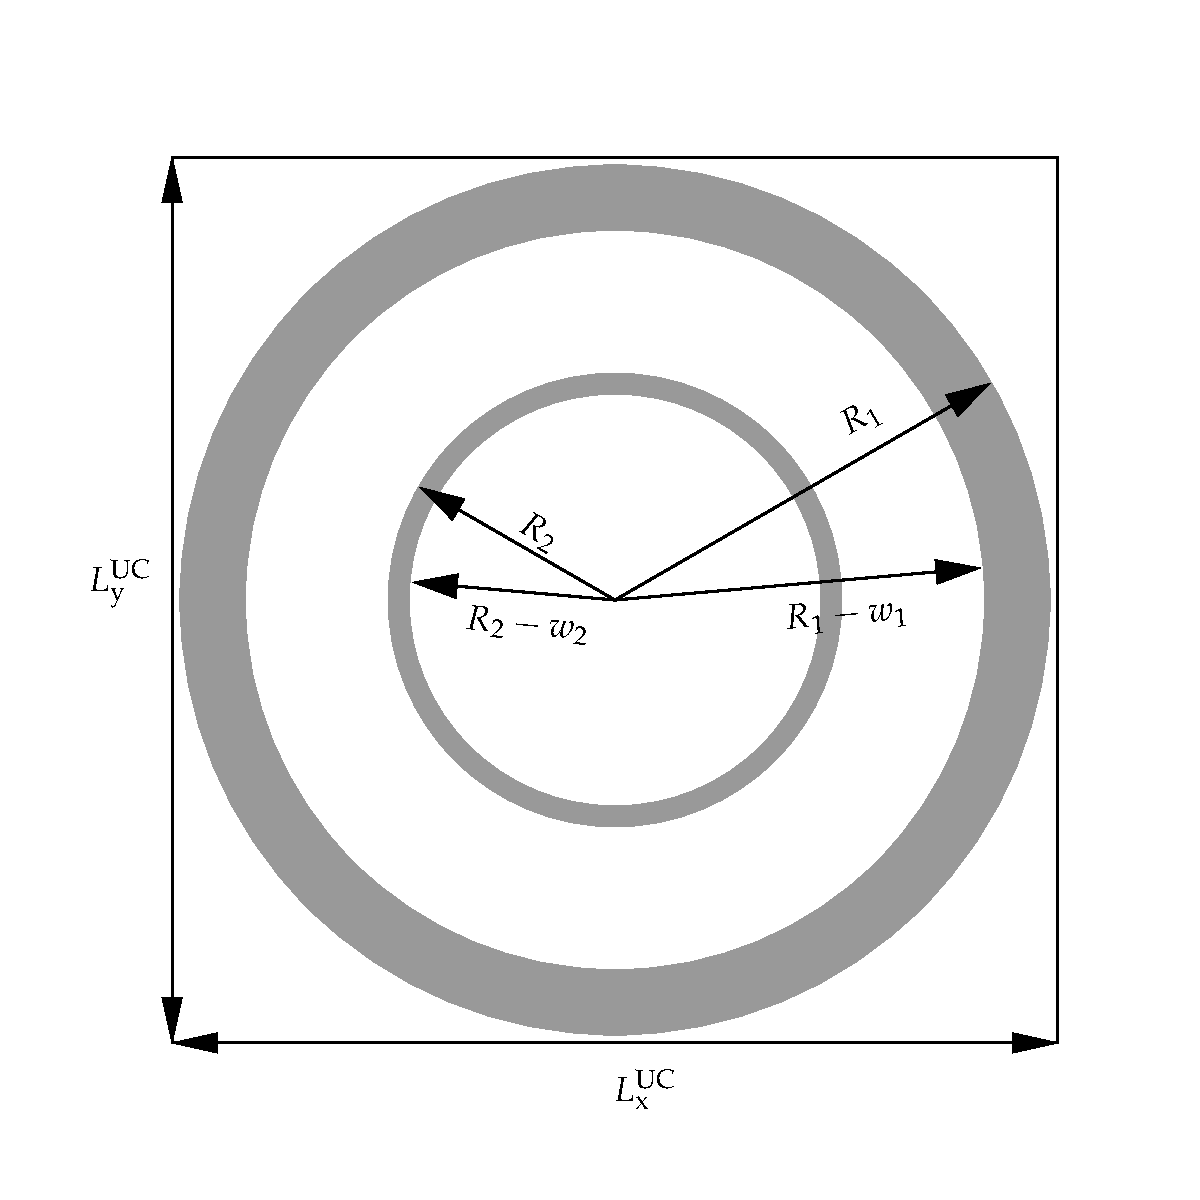
\includegraphics[width=0.75\linewidth]{./media/double_ring_sketch.pdf}
\caption{Two concentric rings of outer radii $R_1$, $R_2$ with widths $w_1$, $w_2$ constitute a metamaterial unit cell with edge lengths of $L_\mathrm{x}^\mathrm{UC}$, $L_\mathrm{y}^\mathrm{UC}$ in $x$- and $y$-direction.}
\label{fig:double_ring_sketch}
\end{figure}

\begin{figure}
\centering
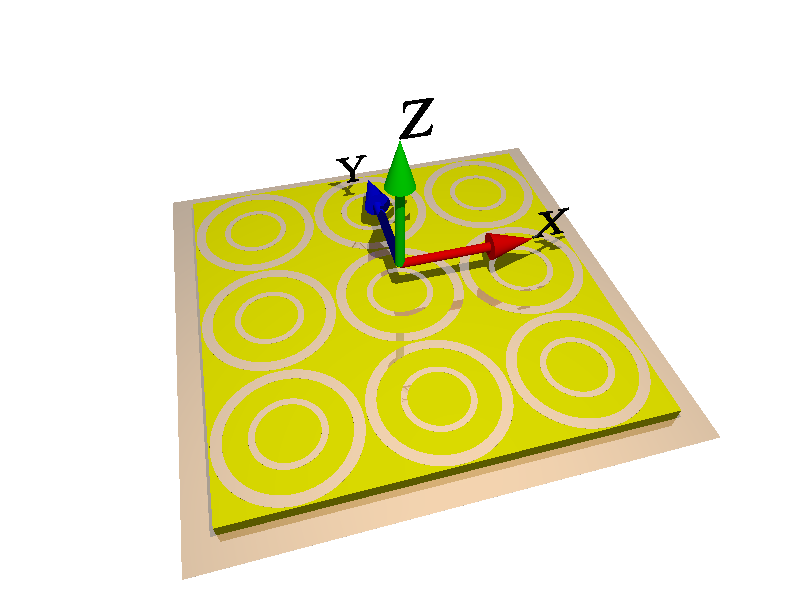
\includegraphics[width=0.75\linewidth]{./media/double_rings.png}
\caption{An artist's view of the suggested metamaterial absorber consisting of a FR4 substrate (yellow) sandwiched between concentric copper rings and a copper backing plane.}
\label{fig:artist_view}
\end{figure}

\subsection{Parameter studies}
In order to find out how the various parameters influence the absorption properties this chapter shows some numerical results for the reflection parameter $S_{11}$.
\capFref{fig:w1_sweep} shows the absolute value of $S_{11}$ as a function of frequency for a fixed outer ring radius of $R_1=9.8$ mm but changing width $w_1$. As we can see there are several additional drops in the scattering parameter including the desired peaks at about 2.4 and 5.2 GHz. Since the 5.2 GHz peak is contributed by the smaller ring changing the width of the larger ring does hardly influence the scattering behaviour at this frequency, whereas at all other frequencies $f<15$ GHz a shift to higher values of $f$ is observed upon an increase of $w_1$.

\begin{figure}
\centering
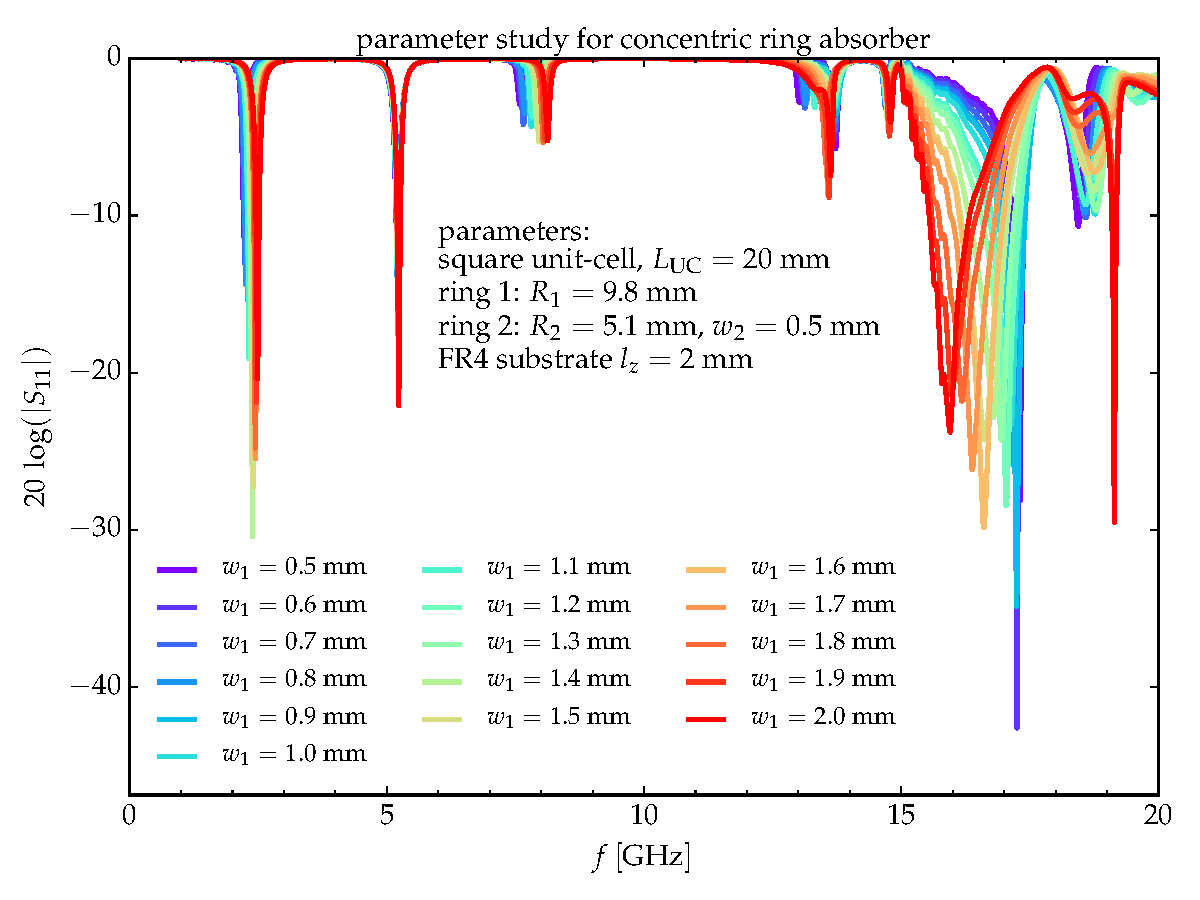
\includegraphics[width=0.75\linewidth]{./media/dual-wifi_absorber_w1.pdf}
\caption{Influence of the larger ring width upon the scattering properties of the concentric ring metamaterial.}
\label{fig:w1_sweep}
\end{figure}

\begin{figure}
\centering
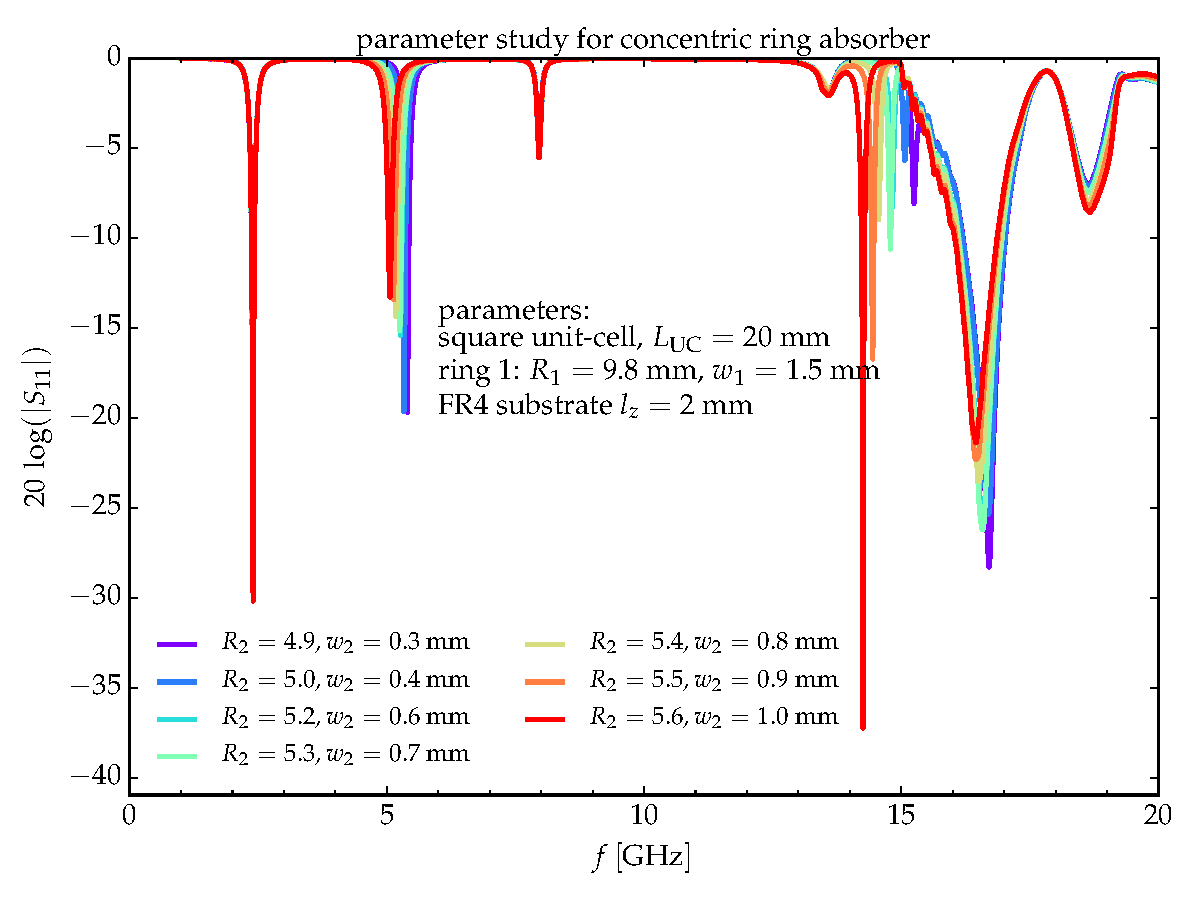
\includegraphics[width=0.75\linewidth]{./media/dual-wifi_absorber_w2.pdf}
\caption{Influence of the smaller ring width upon the scattering properties of the concentric ring metamaterial. In contrast to the study of \Cref{fig:w1_sweep} not the outer, but the inner radius is kept at the value $R_{2i}=4.6$ mm.}
\label{fig:w2_sweep}
\end{figure}

As we would expect a variation of the width of the smaller ring follows the analogous reasoning. \capFref{fig:w2_sweep} exemplifies this behaviour and depicts the absolute value of $S_{11}$ as a function of frequency for a fixed smaller ring radius of $R_{2i}=4.6$ mm but changing width $w_2$. Since this time a second peak, namely the one at approximately 8 GHz doesn't show a dependence upon $w_2$ we can conclude it is associated to a higher harmonic of the larger ring. 

To discriminate the influence of both rings \Cref{fig:single_double_rings} shows the absolute value of the scattering parameter of two isolated rings (solid color lines) and the concentric ring configuration (dashed black line) as functions of frequency.

\begin{figure}
\centering
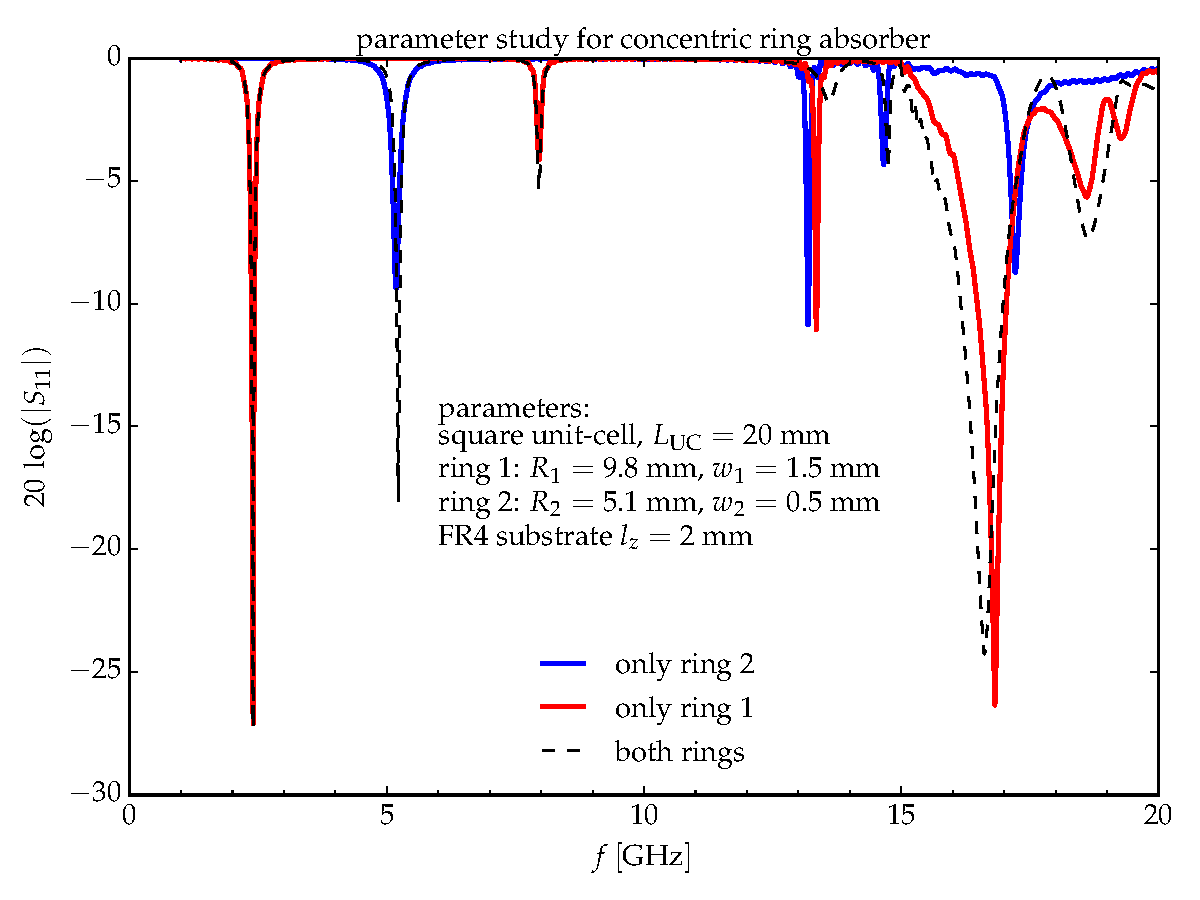
\includegraphics[width=0.75\linewidth]{./media/wifi_absorber_single_double_rings.pdf}
\caption{Comparision of $|S_{11}|$ for an isolated ring 1 with $R_1=9.8$ mm, $w_1=1.5$ mm (red solid), ring 2, $R_2=5.1$ mm, $w_2=0.5$ mm (blue solid) and the concentric configuration (black dashed), where both rings are present.}
\label{fig:single_double_rings}
\end{figure}

To study how the size of the unit-cell influences the position of the absorption 
minima of the double--ring--absorber, \Cref{fig:LUC} shows the position of the two first absorption maxima at about $f_1\approx2.7$ GHz and $f_2\approx 5.5$ GHz as a function of the size of the unit cell, $L^\text{UC}$.
\begin{figure}
\centering
\includegraphics[width=0.75\linewidth]{./media/Einfluss_LUC.pdf}
\caption{Simulated position of the first two absorption maxima of a double ring absorber with $R_1=9.8$ mm, $w_1=1.5$ mm, $R_2=5.1$ mm, $w_2=0.5$ mm as a function of the size of the a-dimension. Metallic parts are chosen to be copper and FR4 is supposed to possess $\Re\left(\epsilon\right)=4.1$ and a loss tangent $\tan\delta = 0.015$.}
\label{fig:LUC}
\end{figure}

What can be observed is that as the size of the unit cell grows, the absorption frequency which can be attributed to the larger ring suffers a shift to higher frequencies. Since this shift tends to saturate as the distance of the outer ring to its neighbours becomes comparable to the ring radius. Therefor we can say that a stronger coupling of neighbouring unit cells leads to an increase of the resonance frequency of the larger ring, whereas the resonance frequency of the smaller ring does not show a significant dependence on the size of the unit cell. This is probably the case since $L^\mathrm{UC}/2 R_2\gtrsim 1.8$ even for the smallest unit cell with $L^\mathrm{UC}=20$ mm, where the beginning of the saturation in \Cref{fig:LUC} is way back.

What is of interest, too is the magnitude of the absorption at the two resonant frequencies as the unit cell grows. \capFref{fig:LUC_absS11} shows this dependence.

\begin{figure}
\centering
\includegraphics[width=0.75\linewidth]{./media/Einfluss_LUC_absS11.pdf}
\caption{Simulated ratio of $|S_{11}(\eta)|/|S_{11}(\eta=1.02)|$ for the first two absorption maxima of a double ring absorber with $R_1=9.8$ mm, $w_1=1.5$ mm, $R_2=5.1$ mm, $w_2=0.5$ mm as a function of the size of the a-dimensional parameter $\eta = L^\mathrm{UC}/2R_1$. Metallic parts are chosen to be made of copper and FR4 is supposed to possess $\Re\left(\epsilon_\mathrm{r}\right)=4.1$ and a loss tangent $\tan\delta = 0.015$.}
\label{fig:LUC_absS11}
\end{figure}


Another important question concerns the impact of the loss taking place in the substrate. \capFref{fig:tand_fi_41} therefore shows the positions of the first two frequencies with minimal $S_{11}$ as a function of $\tan\delta$ of the FR4 substrate at fixed real part $\epsilon_\mathrm{r}^\text{FR4}=4.1$.
It can be observed, that the loss in the substrate does not at all change the resonance frequencies.
In \cref{fig:tand_fi_45} the sweep of $\tan\delta$ without changing anything but the real part of the permittivity to $\epsilon_\mathrm{r}^\text{FR4}=4.5$. Again the resonance frequencies don't show any dependence on the loss since the downwards shift of about 3 \% is within the numerical errors.

\begin{figure}
\centering
\includegraphics[width=0.75\linewidth]{./media/Einfluss_tand_eps_41.pdf}
\caption{Position of the first two absorption frequencies as a function of the loss tangent $\tan\delta$ of FR4 at a fixed value of the real part of the permittivity $\epsilon_\mathrm{r}^\text{FR4}=4.1$.}
\label{fig:tand_fi_41}
\end{figure}
\begin{figure}
\centering
\includegraphics[width=0.75\linewidth]{./media/Einfluss_tand_eps_45.pdf}
\caption{Position of the first two absorption frequencies as a function of the loss tangent $\tan\delta$ of FR4 at a fixed value of the real part of the permittivity $\epsilon_\mathrm{r}^\text{FR4}=4.5$.}
\label{fig:tand_fi_45}
\end{figure}

What can observed, however is that the values of the resonance frequencies in \cref{fig:tand_fi_41} and \cref{fig:tand_fi_45} deviate. 

This naturally leads us to the study of $f_i$ as a function of $\epsilon_\mathrm{r}^\text{FR4}$ in \cref{fig:fi_epsr}. We observe an almost linear dependence of $f_i$ upon $\epsilon_\mathrm{r}^\text{FR4}$ with the same slope for both frequencies. It's worth noting that the shift is relative to the value of $f_i$ at the smallest value of $\epsilon_\mathrm{r}^\text{FR4}$, meaning higher frequencies get shifted more strongly than smaller frequencies. 

\begin{figure}
\centering
\includegraphics[width=0.75\linewidth]{./media/Einfluss_eps.pdf}
\caption{Position of the first two absorption frequencies as a function of $\epsilon_\mathrm{r}^\text{FR4}$ at a fixed value of the loss tangent $\tan\delta=0.015$.}
\label{fig:fi_epsr}
\end{figure}


\subsection{Comparison to measured data}
Due to the promising absorption characteristics of the discussed absorber it has been manufactured and measured experimentally. The magnitude of the measured and simulated values of $S_{11}$ are depicted in 
\newpage
\section{An analytical model of the scattering by rings}
\label{sec:analytical_ring_scattering}
A plane wave of frequency $\omega$ with the elctric field vector pointing along $\unitv{\xi}$ and propagating in the direction of $\mathbf{k}$ can be written: 
\begin{equation}
\mathbf{E}^\text{inc.} (\unitv{r}, t)= E_0 \unitv{\xi} \exp\left[\imag (-\omega t- \mathbf{k}\cdot \mathbf{r})\right].
\label{eqn:Einc_cart}
\end{equation}
In order to describe how a 2d ring scatters waves described by \cref{eqn:Einc_cart} an appropriate coordinate system should be chosen. This could be both, cylindrical ($\rho$, $\phi$, $z$) or spherical coordinates ($r$, $\theta$, $\phi$). From now on we will drop the harmonic time dependence.
In the case of spherical coordinates a complete set of zero-divergence (i. e. sourceless) vector fields are the Hansen multipoles \Cite{Hansen1935}:
\begin{equation}
\mathbf{M}_{\ell m} = \nabla \times \unitv{r} z_\ell(kr) Y_{\ell m}(\theta, \phi),
\label{eqn:HansenM}
\end{equation}
\begin{equation}
\mathbf{N}_{\ell m} = \frac{1}{k}\nabla \times \mathbf{M}_{\ell m}.
\label{eqn:HansenN}
\end{equation}

In \cref{eqn:HansenM} $z_\ell$ is any linear combination of spherical bessel functions $j_\ell(kr)$ and $y_\ell(kr)$ \Cite{DLMF_Bessel} of degree $\ell$. $r$ is the distance from the origin and $k$ the wave number. $Y_{\ell m}$ denote spherical harmonics of degree $\ell$ and order $m$ \Cite{DLMF_SphericalHarmonics}. Their dependence upon the azimut angle $\theta$ and polar angle $\phi$ is understood although not written out explicitly from now on.

Written in terms of $\mathbf{M}_{\ell m}$ and $\mathbf{N}_{\ell m}$ \cref{eqn:Einc_cart} becomes:
\begin{equation}
\unitv{\xi} \exp\left[-\imag  \mathbf{k}\cdot \mathbf{r}\right] =\sum_{\ell,m} \sum_{m'=-\ell}^\ell\mathcal{D}_{m m'}^\ell (\theta_k, \phi_k,0)\big[
m_{\ell, m} \mathbf{M}_{\ell m} +n_{\ell,m} \mathbf{N}_{\ell m}\big].
\end{equation}
Here $\theta_k$ and $\phi_k$ denote the angular coordinates of $\mathbf{k}$ and $\mathcal{D}_{m m'}^\ell$ are Wigner-D matrices in $zxz$ convention. The coefficients $m$ and $n$ can be evaluated to \Cite{Kristensson2014}:
\begin{align}
&& m_{\ell,m} = &\imag^{\ell+1} \delta_{m\pm 1}\sqrt{(2\ell+1)\pi} 
(\unitv{x}\mp\imag \unitv{y})\cdot \unitv{\xi},\\
&& n_{\ell,m} = \pm&\imag^{\ell+1} \delta_{m\pm 1}\sqrt{(2\ell+1)\pi} 
(\unitv{x}\mp\imag \unitv{y})\cdot \unitv{\xi}.
\end{align}

An electromagnetic wave incident on a conducting ring (radius $R$ and width $w$) situated in the $xy$-plane induces currents in the ring which can only exist on the surface of the rings. If the ring possesses zero thickness in $z$-direction and zero width $w$ only currents flowing in $\unitv{\phi}$-direction can exist. Therefore we may write expand the current density responsible for scattered waves in a fourier series in the coordinate $\phi$:
\begin{equation}
\mathbf{j}^\text{scat} = \frac{1}{2\pi R}\sum_{p=-\infty}^\infty \mathrm{e}^{\imag p \phi} \delta(r-R) \delta(\theta-\pi/2) \unitv{\phi}K_p.
\label{eqn:ring_currents}
\end{equation}
Note that \cref{eqn:ring_currents} needs to be extended to include $\unitv{\theta}$ and $\unitv{r}$ components, if the ring possesses a finite thickness or a finite width, respectively. PEC boundary conditions force the components of $\mathbf{E}$ tangential to the surface of the ring to zero and by that determine the coefficients $K_p$.

The fields generated by the current density of \cref{eqn:ring_currents} can be
calculated by using the dyadic Green's function written in terms of vector spherical harmonics\footnote{There is also a freely available version of Gerhard Kristensson's lecture notes on "Spherical Vector Waves" \citep{Kristensson2014}.} \Cite{Kristensson2016}[chapter 7.5]:
\begin{equation}
\dyad{\mathbf{G}}(\mathbf{r},\mathbf{r}') = \imag k \sum_{\ell=1}^\infty \sum_{m=-\ell}^\ell
\mathbf{M}_{\ell m}(\mathbf{r})\otimes\mathbf{M}_{\ell m}^*(\mathbf{r}')+
\mathbf{N}_{\ell m}(\mathbf{r})\otimes\mathbf{N}_{\ell m}^*(\mathbf{r}'),
\label{eqn:Greens_Dyadic}
\end{equation}
where the vectorfield depending on the position vector with the smaller magnitude, $r_<=\min\left(r, r'\right)$, is to be understood to depend on regular spherical bessel functions $j_\ell(kr_<)$ whereas the other vectorfield possesses a dependence on the radial coordinate $r_>=\max\left(r, r'\right)$ via outgoing\footnote{The term outgoing is owing to the choice of the $\exp\left(-\imag\omega t\right)$ time dependence.} spherical hankel functions of the first type, $h_\ell^{(1)}(kr_>)$.
The asterix $^*$ means complex conjugation. With the aid of \cref{eqn:Greens_Dyadic} the scattered electric field can be calculated via:
\begin{equation}
\mathbf{E}^\text{scat}(\mathbf{r}) = \int_{\mathcal{R}^3}  \rd \mathbf{r}' 
\dyad{\mathbf{G}}(\mathbf{r},\mathbf{r}') \cdot \mathbf{j}^\text{scat}(\mathbf{r}').
\label{eqn:E_scattered}
\end{equation}

The scattered field of \cref{eqn:E_scattered} can be therefore cast in the form:
\begin{equation}
\mathbf{E}^\text{scat}(\mathbf{r}) = \imag k \sum_{\ell=1}^\infty  \sum_{m=-\ell}^\ell
I_{\ell m}^\textbf{(M)}\mathbf{M}_{\ell m}(\mathbf{r})+
I_{\ell m}^\textbf{(N)}\mathbf{N}_{\ell m}(\mathbf{r})
\label{eqn:Escat}
\end{equation}
with the expansion coefficients
\begin{align}
I_{\ell m}^\text{(M)} = \int \rd^3\mathbf{r}' \mathbf{M}^*_{\ell m}(\mathbf{r}')\cdot
\mathbf{j}^\textbf{scat}(\mathbf{r}'),\\
I_{\ell m}^\text{(N)} = \int \rd^3\mathbf{r}' \mathbf{N}^*_{\ell m}(\mathbf{r}')\cdot
\mathbf{j}^\textbf{scat}(\mathbf{r}'),
\end{align}
where the Hansen multipoles have to be written with regular spherical bessel function $j_\ell(kr)$. The above integrals can be evaluated in closed form, if \cref{eqn:ring_currents} is inserted for the scattered current density $\mathbf{j}^\text{scat}$ yielding:
\begin{align}
\left.I_{\ell m}^\textbf{(M)} = \delta_{p m}\frac{j_\ell(kR)}{\sqrt{\ell(\ell+1)}} \left[-K_p\frac{\displaystyle\rd}{\rd \theta}P_{\ell}^{(m)}(\cos(\theta))
\right]\right \vert_{\theta=\pi/2},\\
\left.I_{\ell m}^\textbf{(N)} =  \delta_{p m} 
\frac{\frac{\rd}{\rd (kR)}\left[kR j_\ell(kR)\right]}{kR\sqrt{\ell(\ell+1)}}\left[-\imag m K_p
P_\ell^{(m)}(\cos(\theta)) \right]\right\vert_{\theta=\pi/2}.
\end{align}
The associated Legendre polynomials and their derivative can be written \Cite{Leong1997}:
\begin{align}
\frac{\rd}{\rd \theta}P_\ell^{(m)}(0) =\left\{\ontop{}{}{
-\sin\big((\ell+m)\pi/2\big)\dfrac{2^{m+1}\Gamma\big((l+m)/2+1\big)}{\sqrt{\pi}\Gamma\big((l-m+1)/2\big) }
\quad : \quad (l+m)\%2=1}{\quad0\quad: \quad\text{otherwise}}\right\},
\label{eqn:Plm0diff}
\\\left\{
P_\ell^{(m)}(0) = \ontop{}{}{\cos\big((l+m)\pi/2\big)\dfrac{2^m \Gamma\big((n+m+1)/2\big)}{\sqrt{\pi}\Gamma\big((n-m)/2+1\big)}\quad:\quad (l+m)\%2=0}{0\quad:\quad \text{otherwise}}\right\}.
\label{eqn:Plm0}
\end{align}
If we are just interested in the scattered field and not the current distribution in the rings, we find the $I$-coefficients by requiring that for each occuring term proportional to $\mathbf{M}_{\ell,m}$ and $\mathbf{N}_{\ell,m}$ in the expansion of the incoming field the respective terms on the right-hand side of \cref{eqn:E_scattered} must ensure that 
\begin{align}
\left(
E_0^\text{inc}\left[
\begin{matrix}
\mathbf{M}_{\ell,m}^\text{reg} \\
\mathbf{N}_{\ell,m}^\text{reg}
\end{matrix}\right]
+
\imag k \left[\begin{matrix}
I_{\ell m}^\textbf{(M)}\mathbf{M}_{\ell,m}^\text{out} \\
I_{\ell m}^\textbf{(N)}\mathbf{N}_{\ell,m}^\text{out}
\end{matrix}\right]\right) \cdot 
\unitv{\phi}\left.\right\vert_{\theta=\pi/2,r=R} = 0
\end{align}

\subsection{Perpendicular incidence, perfectly conducting rings}
At perpendicular incidence the cylindrical symmetry of the rings allows to choose the polarization in $\unitv{x}$-direction without loss of generality. Therefore \cref{eqn:Einc} becomes:
\begin{equation}
\mathbf{E}^\text{inc.} (z, t)= \unitv{x} \exp\left[\imag (-\omega t- k\cdot z)\right].
\label{eqn:Ex}
\end{equation}
Henceforth the time-dependence $\exp(-\imag \omega t)$ will be suppressed. To satisfy the boundary conditions
\begin{align}
\left.\left(\mathbf{E}^\text{inc.}+\mathbf{E}^\text{scat}\right)\times \unitv{r}\right\vert_{\theta=\pi/2, r=R} = 0,
\label{eqn:Etan}\\
\left.\left(\mathbf{H}^\text{inc.}+\mathbf{H}^\text{scat}\right)\times \unitv{r}\right\vert_{\theta=\pi/2, r=R} = 0,
\label{eqn:Htan}
\end{align}
for the field components transverse to the rings we expand \cref{eqn:Ex} in Hansen multipoles \cite{Kristensson2014}[p. 44 ff.]:
\begin{equation}
\mathbf{E}^\text{inc.} = \sqrt{(2\ell+1)\pi}\sum_{\ell=1}^\infty \imag^{\ell+1}\ 
\big( \mathbf{M}_{\ell m} \pm \imag \mathbf{N}_{\ell m}\big) \delta_{m \pm 1}
\label{eqn:Einc}
\end{equation}
and have to take care that the $\unitv{\phi}$- and $\unitv{\theta}$-components of the total fields satisfy \cref{eqn:Etan,eqn:Htan}. Supposing for the moment, that the ring is small as compared to the wavelength, we can restrict the sums in \cref{eqn:Escat} to $\ell=1$. This assumption leads to  $I^\text{(M)}_{1,\pm 1}=0$ (see \cref{eqn:Plm0diff}), whereas $I^\text{(N)}_{1,\pm 1}$ (see \cref{eqn:Plm0}) survives for $|m|=1$.
\begin{align}
\left[
\renewcommand\arraystretch{1.4}\begin{matrix}
I_{1,1}^\text{(M)} \\
I_{1,0}^\text{(M)} \\ 
I_{1,-1}^\text{(M)}
\end{matrix} \right]=
\frac{j_1(kR)}{\sqrt{2}} \left[ 
\renewcommand\arraystretch{1.4}\begin{matrix}
0 \\ K_0 \\ 0
\end{matrix}
\right]
\\
\left[
\renewcommand\arraystretch{1.4}\begin{matrix}
I_{1,1}^\text{(N)} \\
I_{1,0}^\text{(N)} \\ 
I_{1,-1}^\text{(N)}
\end{matrix} \right] =  \frac{\frac{\rd}{\rd (kR)}\left[kR j_1(kR)\right]}{kR\sqrt{2}} 
\left[
\renewcommand\arraystretch{1.4}\begin{matrix}
-K_1\\0\\+K_{-1}
\end{matrix}
\right]
\end{align}

We observe, that in order to match the boundary conditions the coefficients $I_{\ell m}^\text{(M)}$ and $I_{\ell m}^\text{(N)}$ resemble Mie's coefficients for a perfectly conducting sphere of radius $R$, $b_\ell$ and $a_\ell$. 
The fact that on the thin ring no currents in the $\unitv{\theta}$-direction leads to the vanishing magnetic dipole polarizability in the $xy$-plane i. e. zero terms $I_{\ell, \pm 1}^\text{(M)}$ and a vanishing electric dipole polarizability in the $\unitv{z}$-direction $I_{\ell, 0}^\text{(N)}$.

\subsection{xy-periodic array of thin rings}
Building upon the results of the last section we can discuss the scattering of a periodic arrangement of rings in the $xy$-plane by forcing the expansion coefficients $Q^\text{TM}$ and $Q^\text{TE}$ of the total electric field to be eigenfunctions of the translationoperators $\mathcal{P}_x$ and $\mathcal{P}_y$. This is necessary because the fields in the periodic structure must satisfy:
\begin{equation}
\mathbf{E}\left(\mathbf{r}+m L \unitv{x}+
n L \unitv{y}\right)=
\mathbf{E}\left(\mathbf{r}\right).
\end{equation}
For any choice of the whole numbers $m, n\in \mathbb{Z}$. Therefore we can write
\begin{equation}
\mathbf{E}\left(\mathbf{r}\right) = 
\exp\left(\imag \frac{2\pi}{L}x\right) \exp\left(\imag \frac{2\pi}{L}y\right)\mathbf{\tilde{E}}\left(\mathbf{r}\right),
\end{equation}
where $\mathbf{\tilde{E}}(\mathbf{r})$ is the field in a single unit-cell. Each of the exponential factors can be expanded in the fashion:
\begin{equation}
\exp\left(\imag\mathbf{k}\cdot \mathbf{r}\right) = 4\pi \sum_{\ell=0}^\infty \sum_{m=-\ell}^\ell
\imag^\ell j_\ell(kr) Y_{\ell m}(\unitv{r}) Y_{\ell m}^*(\unitv{k}),
\end{equation}
where the arguments $\unitv{r}$, $\unitv{k}$ of the spherical harmonics are a shortcut for the dependence upon the angles $\theta$, $\phi$ of the position vector $\mathbf{r}$ and $\theta_\mathrm{k}$, $\phi_\mathrm{k}$ of the wave vector $\mathbf{k}$. Substituting $\mathbf{k}=\frac{2\pi}{L}\unitv{x}$ we end up with:
\begin{align}
&& \nonumber
\exp\left(\imag \frac{2\pi}{L} x\right) &= 4\pi \sum_{\ell=0}^\infty \sum_{m=-\ell}^\ell
\imag^\ell j_\ell\left(\frac{2\pi r}{L}\right) Y_{\ell m}(\theta, \phi) Y_{\ell m}^*\left(\frac{\pi}{2}, 0\right) \\
&& &= 4\pi N_{\ell m} \sum_{\ell=0}^\infty \sum_{m=-\ell}^\ell
\imag^\ell j_\ell\left(\frac{2\pi r}{L}\right) Y_{\ell m}(\theta, \phi)
P_{\ell m}(0).
\label{eqn:xperiodicity}
\end{align}
This sum contains only terms of pairs $(\ell,m)$ with even $\ell+m$ (see \cref{eqn:Plm0}). If we collect both, the exponential depending on $x$ and $y$ we can combine them to:
\begin{equation}
\exp\left(\imag \frac{2\pi}{L} (x+y)\right) = 4\pi \sum_{\ell=0}^\infty \sum_{m=-\ell}^\ell
\imag^\ell j_\ell\left(\frac{2\pi r}{L}\right) Y_{\ell m}(\theta, \phi) Y_{\ell m}^*\left(\frac{\pi}{2}, \pi/4\right).
\end{equation}

In total we end up with the boundary condition:
\begin{equation}
\left[\mathbf{E}^\text{inc}+\exp\left(\imag \frac{2\pi}{L}(x+y)\right)\mathbf{E}^\text{scat}\right] \cdot \unitv{\phi}\big|_{r=R} = 0
\end{equation}
\newpage
\section{Scattering coefficients of a plane surface}
The scattering coefficients for an electromagnetic wave of angular frequency $\omega$ propagating in medium 1 with refractive index $n_1=\sqrt{\epsilon_1\mu_1}$ incident on a medium with $n_2 = \sqrt{\epsilon_2\mu_2}$ 
\begin{equation}
r^\text{TE}=\frac{k_1 \mu_2 - k_2 \mu_1}{k_1 \mu_2 + k_2 \mu_1}
\label{eqn:FresnelTE}
\end{equation}
\begin{equation}
r^\text{TM}=\frac{k_1 \epsilon_2 - k_2 \epsilon_1}{k_1 \epsilon_2 + k_2 \epsilon_1}
\label{eqn:FresnelTM}
\end{equation}
where $k_i = \sqrt{k_\perp^2 - n_i^2\omega^2/c^2}$ and $k_\perp$ is modulus of the in-plane wave vector.

\newpage
\section{Transmission Line Theory for a single ring}
Consider a square unit-cell of edge length $L$ and a copper ring of outer Radius $R$ and width $w$ in it.
The ring can be modelled by transmission line theory to behave as a series RLC-circuit. 
The single ring has an inductance of:
\begin{equation}
L = \mu_0 (R-w) \ln\left(
\frac{16(R-w)}{w}-2
\right)
\end{equation}
\newpage 
\section{Useful identities}
\subsection{Symmetry}
Consider the following integral occurring in xy-periodic structures:

\begin{equation}
I^{\mathrm{Y\mathbf{X}\mathbf{X}}}_{123} \equiv \int \rd \Omega \, Y_{\ell_1, m_1} \mathbf{X}_{\ell_2, m_2}\cdot \mathbf{X}^*_{\ell_3,m_3}.
\label{eqn:YXX_integral}
\end{equation}

Without the spherical harmonic $Y_{\ell_1,m_1}$ the obove integral would have yielded
1, since the VSH $\mathbf{X}_{\ell, m}$ is normalized with respect to integration over the surface of the unit-sphere and $\mathbf{X}_{\ell,m},\mathbf{W}_{\ell,m}$ form an orthogonal set of zero-divergence vectorfields. 

Lets carry out the dot product of the two vector spherical harmonics:
\begin{equation}
I^{\mathrm{Y\mathbf{X}\mathbf{X}}}_{123} =\frac{1}{\sqrt{\ell_2(\ell_2+1)\ell_3(\ell_3+1)}}\int \rd \Omega\, 
Y_{\ell_1,m_1}\left[
\frac{m_2 m_3}{\sin^2\theta} Y_{\ell_2,m_2} Y^*_{\ell_3, m_3}
+\partial_\theta Y_{\ell_2,m_2}\partial_\theta Y^*_{\ell_3,m_3}
\right]
\label{eqn:YXX_integral_split}
\end{equation}
\subsection{Vector Multipole Fields}
In spherical coordinates the vectorial Helmholtz equation possesses the set of
solutions:
\begin{align}
&& \mathbf{X}_{\ell m} &= \frac{1}{\sqrt{\ell(\ell+1)}} \left[
\unitv{\theta} \frac{1}{\sin(\theta)} \frac{\partial}{\partial \phi} Y_{\ell m} -
\unitv{\phi} \frac{\partial}{\partial \theta} Y_{\ell m}
\right], \label{eqn:Xlm}\\
&& \mathbf{W}_{\ell m} &= \frac{1}{\sqrt{\ell(\ell+1)}} \left[
\unitv{\theta} \frac{\partial}{\partial \theta} Y_{\ell m} +
\unitv{\phi} \frac{1}{\sin(\theta)} \frac{\partial}{\partial \phi} Y_{\ell m} 
\right], \label{eqn:Wlm}\\
&& \mathbf{L}_{\ell m} &= \unitv{r} Y_{\ell m},\label{eqn:Llm}
\end{align}
which are orthonormal upon integration over the unit-sphere. With \cref{eqn:Xlm,eqn:Wlm,eqn:Llm} one can construct the zero-divergence Hansen-Multipoles:
\begin{align}
&& \mathbf{M}_{\ell m} &= \mathbf{X}_{\ell m} z_\ell(kr), \\
&& \mathbf{N}_{\ell m} &= \sqrt{\ell(\ell+1)} \frac{z_\ell(kr)}{kr} \mathbf{L}_{\ell m}+
\frac{\left[kr z_\ell(kr)\right]'}{kr}\mathbf{W}_{\ell m} z_\ell(kr) \label{eqn:NlmVSH}
\end{align}
where the parenthesis in \cref{eqn:NlmVSH} denotes differentiation with respect to the argument $kr$.


\subsection{Vector Multipole-Translations}
Suppose given is a multipole field vector:
\begin{equation}
\ket{\mathbf{E}_m^A} = \left[
Q^\text{M}_{\ell_\text{min},m}, Q^\text{M}_{\ell_\text{min}+1,m},...,
Q^\text{M}_{\ell_\text{max},m};
Q^\text{E}_{\ell_\text{min},m}, Q^\text{E}_{\ell_\text{min}+1,m},...,
Q^\text{E}_{\ell_\text{max},m}
\right]^T
\end{equation}
given in a frame of reference $A$ with magnetic and electric multipole coefficients $Q^\text{M}_{\ell,m}, Q^\text{E}_{\ell,m}$ indexed by the angular momentum number $\ell$ and its z-projection $m$. $\ell_\text{min}$ and $\ell_\text{max}$ shall denote the minimum angular momentum involved in the $m$-block, $\ell_\text{min}=\max(|m|,1)$ and $\ell_\text{max}$ is the maximum angular momentum we are interested in.

If we want to know the respective coefficients in a second frame of refernence, $B$ which is shifted by the vector $\mathbf{d}=\pm d \mathbf{z}$\footnote{Note that translations in the z-direction are especially simple since $m$ is conserved and that every frame of reference can always be rotated such that the vector $\mathbf{d}$ points along the $z$-axis.} relative to $A$ we apply the following translation relation:
\begin{equation}
\ket{\mathbf{E}_m^B} = \mathbb{V}^\text{m} \ket{\mathbf{E}_m^A},
\end{equation}
where $\mathbb{V}^\text{m}$ is a $2\times 2$ block-matrix
\begin{equation}
\mathbb{V}^m = \left[
\begin{matrix}
\mathbb{V}^{\mathrm{PP},m} & \mathbb{V}^{\mathrm{PQ},m} \\
\mathbb{V}^{\mathrm{PQ},m} & \mathbb{V}^{\mathrm{PP},m}
\end{matrix}
\right]
\end{equation}
with polarization conserving (mixing) entries PP (PQ) \Cite{Wittmann1988}:
\begin{align}
&&\left(\mathbb{V}^{\mathrm{PP},m}\right)_{\ell_1,\ell_2} &= 
C^{m,\pm}_{\ell_1,\ell_2} \sum_{\alpha=|\ell_1-\ell_2|}^{\ell_1+\ell_2}
D^m_{\ell_1,\ell_2,\alpha}(kd) 
\big[\ell_1(\ell_1+1) + \ell_2(\ell_2+1)-\alpha(\alpha+1)\big]\frac{1}{2},\\
&&\left(\mathbb{V}^{\mathrm{PQ},m}\right)_{\ell_1,\ell_2} &= \mp \imag m kd\,
C^{m,\pm}_{\ell_1,\ell_2} \,  \sum_{\alpha=|\ell_1-\ell_2|}^{\ell_1+\ell_2}
D^m_{\ell_1,\ell_2,\alpha}(kd).
\end{align}
We introduced the abbreviations:
\begin{align}
&&C^{m,\pm}_{\ell_1,\ell_2} &= \frac{(-1)^m (\pm \imag)^{\ell_1-\ell_2}2\sqrt{\pi}}
{\sqrt{\ell_1(\ell_1+1)\ell_2(\ell_2+1)}},\label{eqn:Ccoeff}
\\
&&D^m_{\ell_1,\ell_2,\alpha}(kd) &= \imag^\alpha \sqrt{2\alpha+1} z_\alpha(kd)
\mathrm{Y}^{\ell_1, \ell_2, \alpha}_{m,-m,0}\label{eqn:Dcoeff}
\end{align}
with the Gaunt-coefficients $\mathrm{Y}^{\ell_1 \ell_2 \alpha}_{m,-m,0}$, an integral of three spherical harmonics over the surface of the unit-sphere:
\begin{equation}
\mathrm{Y}^{\ell_1, \ell_2, \alpha}_{m,-m,0} = \int_{\partial B_1(0)} \rd \Omega \,
Y_{\ell_1,m}(\theta,\phi) Y_{\ell_2,-m}(\theta,\phi) Y_{\alpha,0} (\theta,\phi)
\label{eqn:Gaunt}
\end{equation}
and spherical bessel functions $z_\alpha(kd)$ which are to be understood to be either regular ($z_\alpha = j_\alpha$) or outgoing ($z_\alpha = h^{(1)}_\alpha$) depending on whether the orgin is inclosed in the region where the field is to be evaluated or not.  \capEref{eqn:Ccoeff}  depends upon the the sign of the translation, with $+$ for translations in positive $z$-direction and $-$ for translations in the opposite direction.





\newpage


%%% name of the bibliography file without .bib
%%% e.g.: literatur.bib -> 

\printbibliography


\end{document}
